
%\section{Pasos para configurar smartphone Android en modo Desarrollador}

\begin{frame}
\frametitle{Crear un primer proyecto (1)}  
\begin{columns}
\column{0.50\linewidth}
\begin{itemize}
\item Buscar el icono de la aplicacion y dar doble click
\item En caso de que requiera algunas actualizaciones, ser paciente, puede tardar.
\item Aparecera una ventana como la mostrada, seleccionar la opci\'on ``New project''
\end{itemize}
\column{0.50\linewidth}
\begin{center}
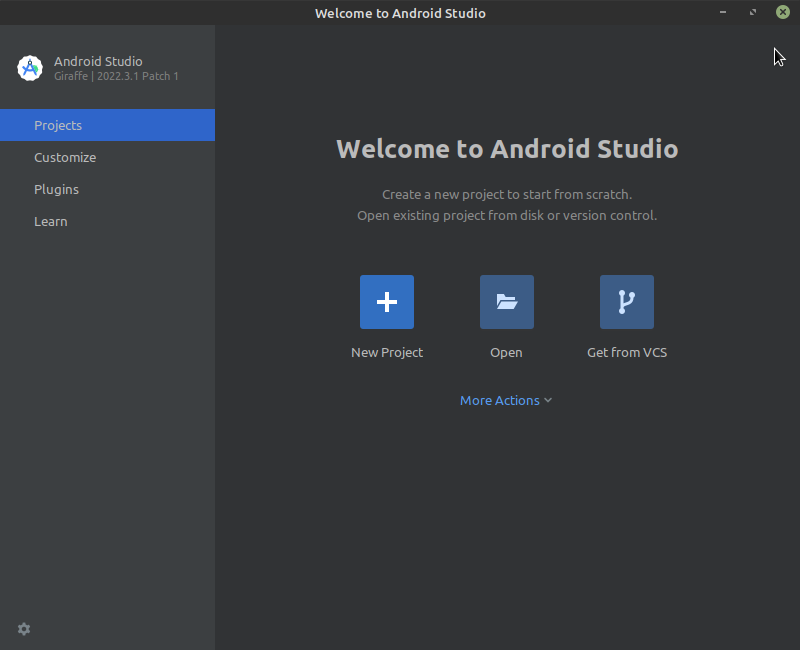
\includegraphics[width=0.95\linewidth]{01_PasosCrearProyectoAndroidStudio/AndroidStudio01.png}    
\end{center}
\end{columns}
\end{frame}

\begin{frame}
\frametitle{Crear un primer proyecto (2)}  
\begin{columns}
\column{0.50\linewidth}
\begin{itemize}
\item Existen varios tipos de dispositivos para los que pueden crearse proyectos. Por defecto nos ubica en el primer grupo (Phone and Tablet)
\item Seleccionar tipo de proyecto  ``Empty Views Activity'' y dack click en Next
\end{itemize}
\column{0.50\linewidth}
\begin{center}
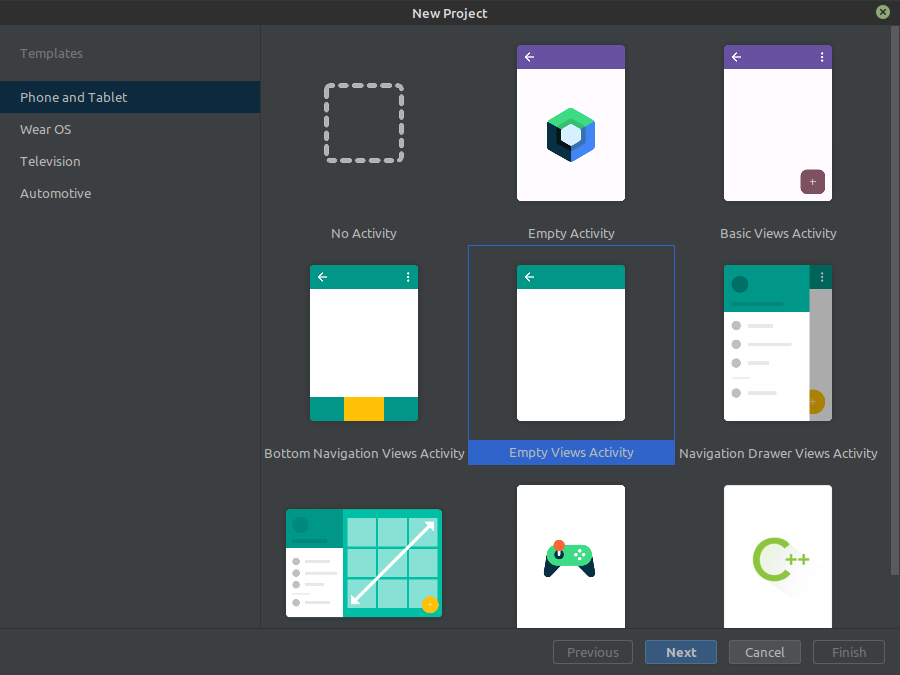
\includegraphics[width=0.95\linewidth]{01_PasosCrearProyectoAndroidStudio/AndroidStudio02.png}    
\end{center}
\end{columns}
\end{frame}

\begin{frame}
\frametitle{Crear un primer proyecto (3)}  
\begin{columns}
\column{0.50\linewidth}
\begin{itemize}
\item Dejar los valores por defecto, solo se suguiere cambiar el nombre del proyecto
\item \textbf{Debe estar seleccionado como lenguaje Kotlin}. De estar seleccionado uno diferente, cambiar
\item Presionar el boton Finish
\end{itemize}
\column{0.50\linewidth}
\begin{center}
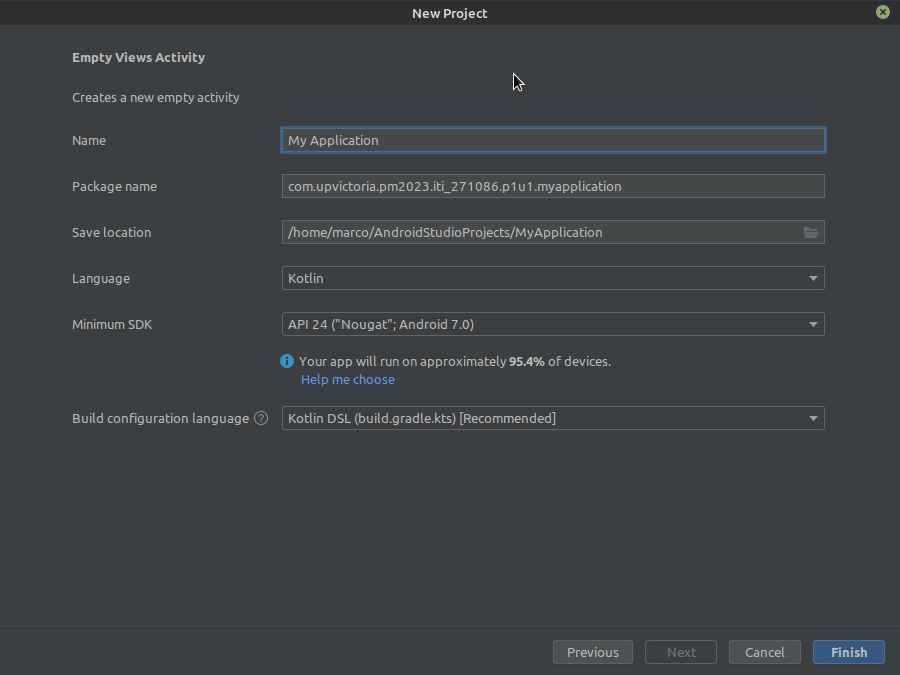
\includegraphics[width=0.95\linewidth]{01_PasosCrearProyectoAndroidStudio/AndroidStudio03.png}    
\end{center}
\end{columns}
\end{frame}

\begin{frame}
\frametitle{Crear un primer proyecto (4)}  
\begin{columns}
\column{0.50\linewidth}
\begin{itemize}
\item La primera vez que se crea un proyecto, puede requerir la descarga de archivos necesarios. Le recomiendo ser paciente
\item Ya una vez que el proyecto fue creado, aparece la ventana mostrada
\end{itemize}
\column{0.50\linewidth}
\begin{center}
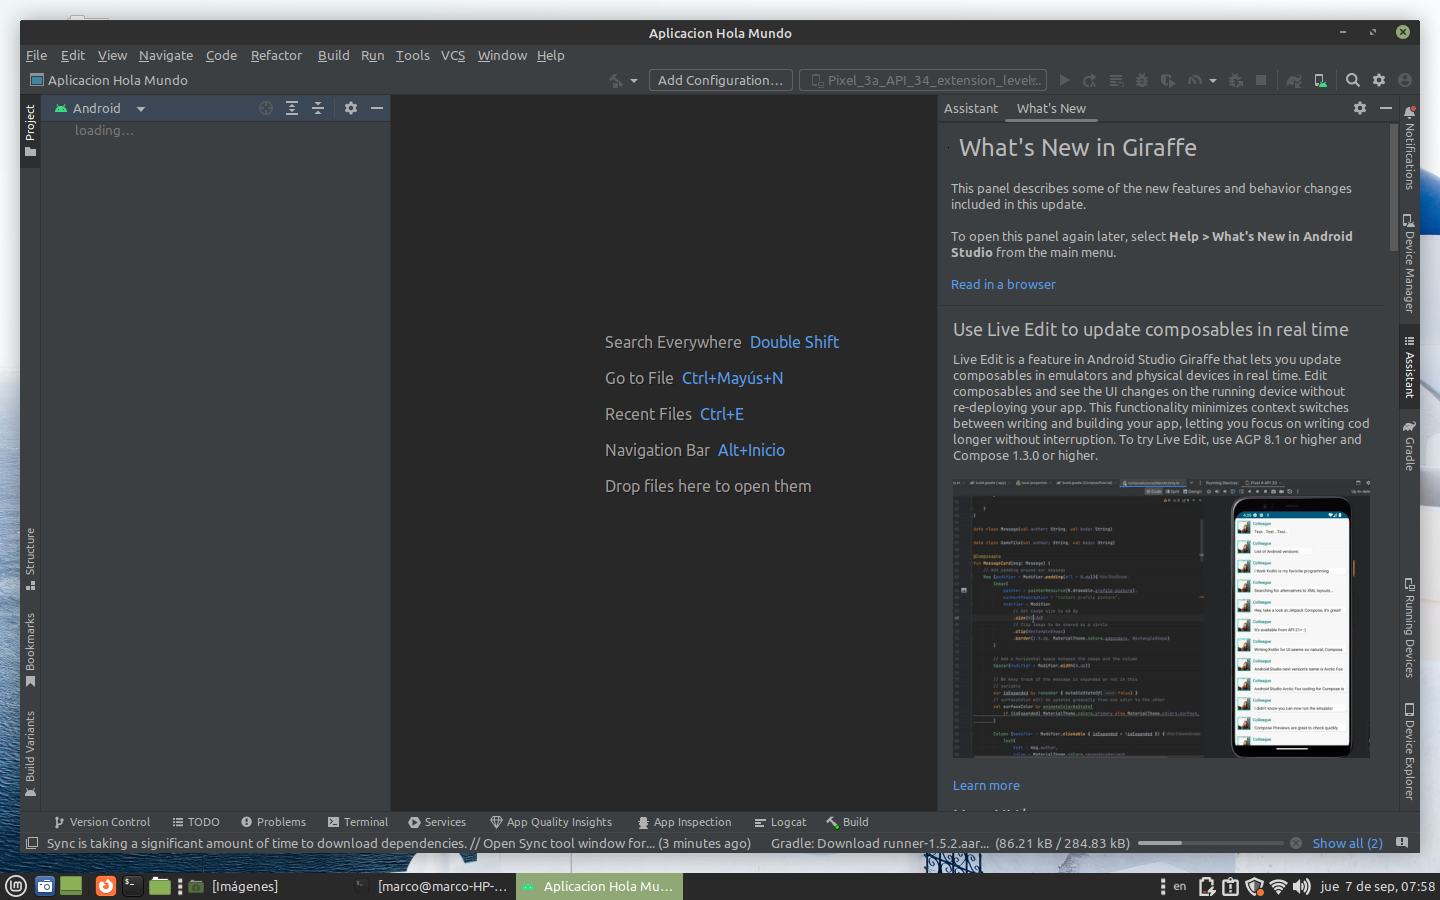
\includegraphics[width=0.95\linewidth]{01_PasosCrearProyectoAndroidStudio/AndroidStudio04.png}    
\end{center}
\end{columns}
\end{frame}


\begin{frame}
\frametitle{Ejecutar proyecto en telefono inteligente} 
\begin{columns}

\column{0.75\linewidth}
\begin{itemize}
\item Una vez conectado el telefono, debe aparecer el modelo en la parte superior (lado derecho) de tu proyecto de Android Studio
\item Para instalar la aplicacion en el telefono, deber dar click en una flecha verde justo a un lado de nombre del telefono (sean pacientes, puede tardar un poco la primera vez)
\end{itemize}
\begin{center}
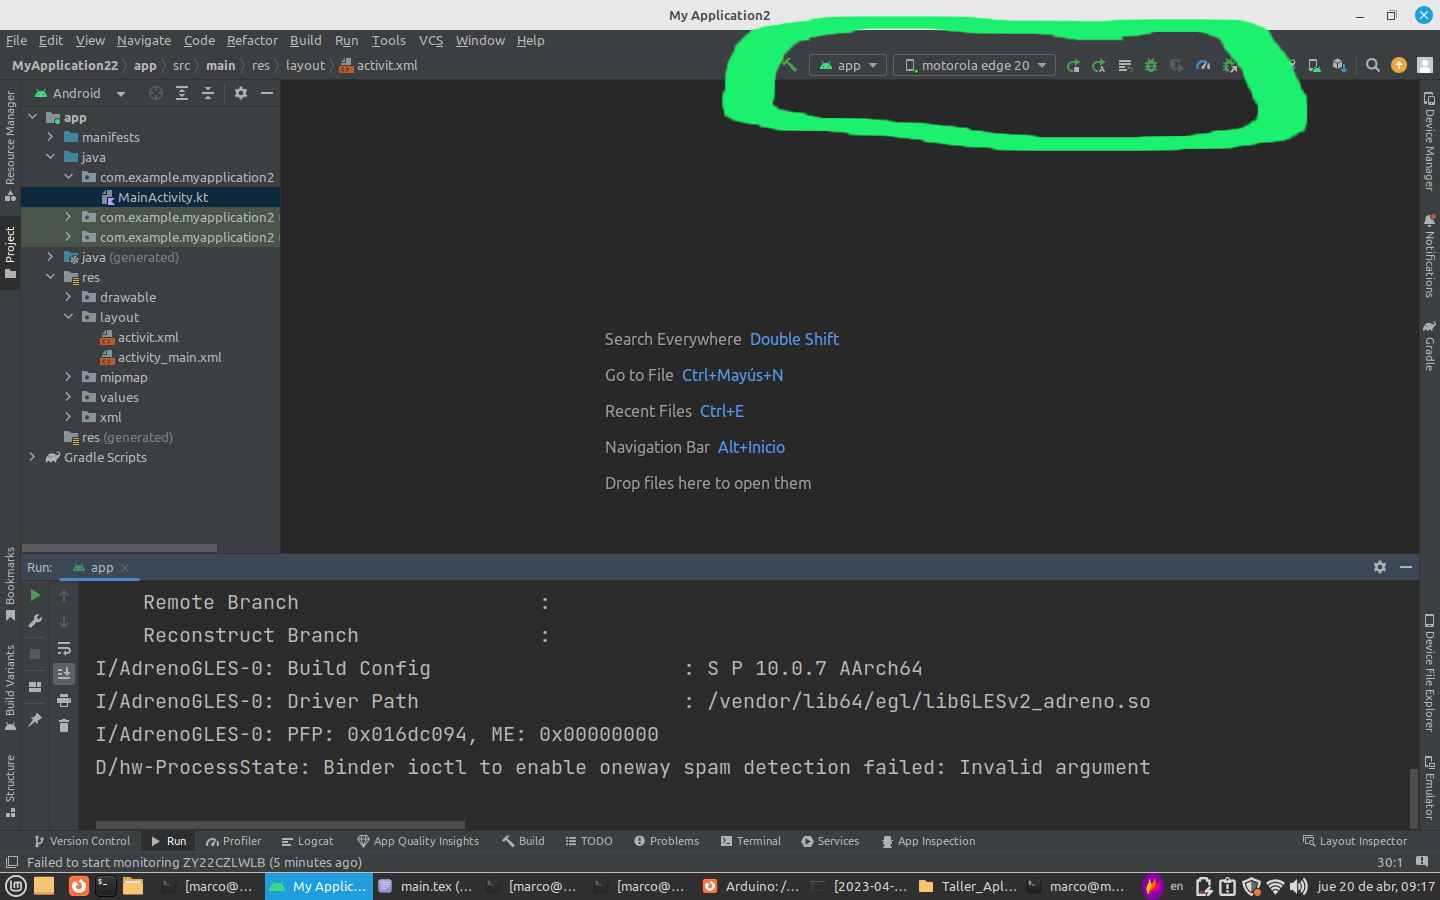
\includegraphics[width=0.65\linewidth]{01_PasosCrearProyectoAndroidStudio/AndroidStudio_SmartphoneReconocido.png}    
\end{center}
\column{0.25\linewidth}
\begin{center}
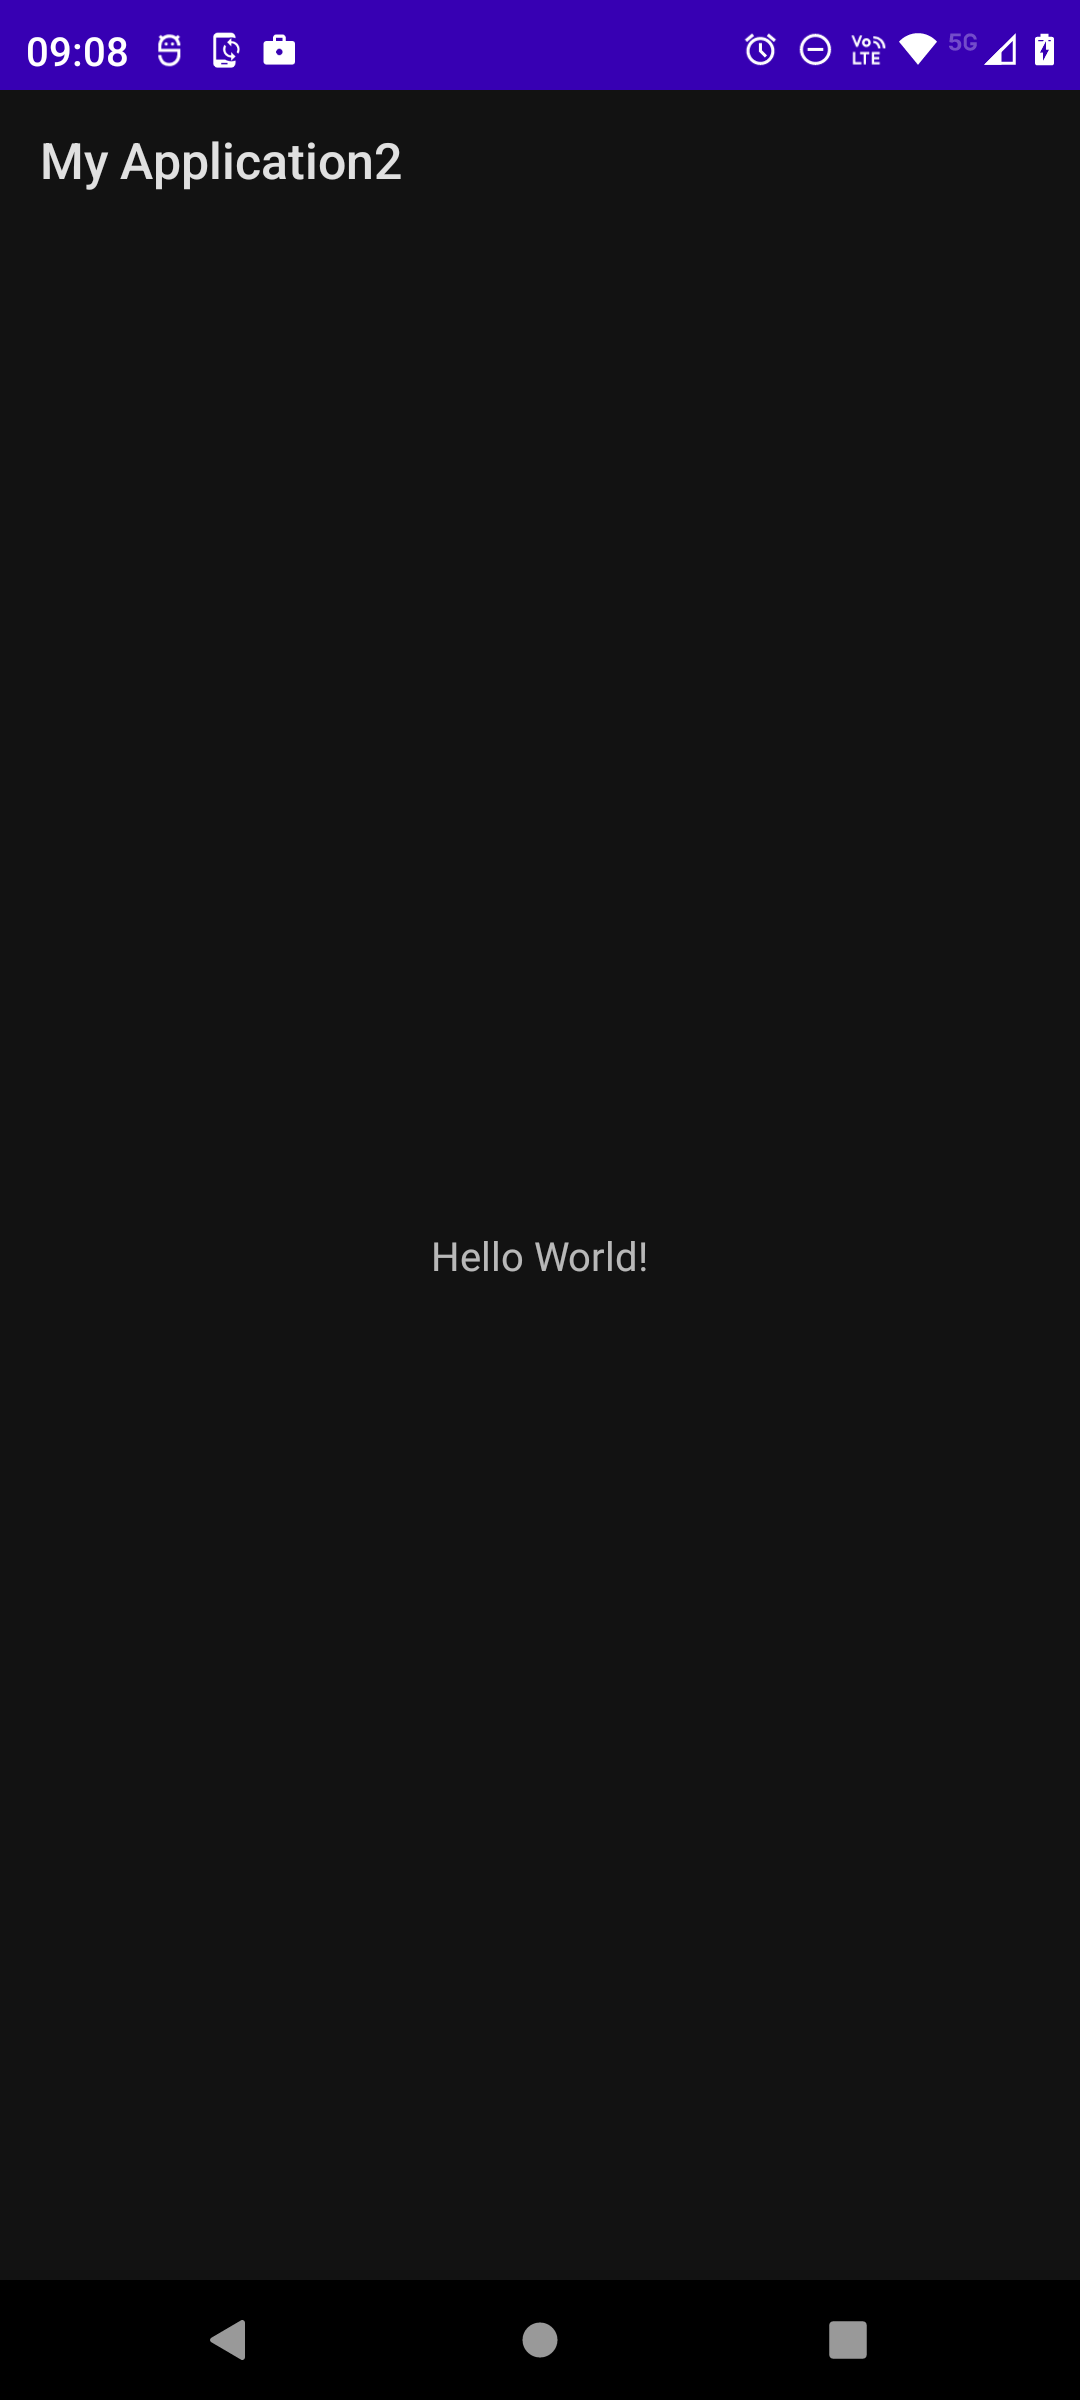
\includegraphics[width=0.95\linewidth]{01_PasosCrearProyectoAndroidStudio/Etapa1_fase1.png}    
\end{center}
\end{columns} 
\end{frame}



